% ----------------------------------------------------------------
% Article Class (This is a LaTeX2e document)  ********************
% ----------------------------------------------------------------
\documentclass{article}
\usepackage[english]{babel}
\usepackage{styfiles/proof, styfiles/code, amsmath,amsthm}
\usepackage{amssymb}  % for "\leadsto"
\usepackage{bbold}%for typeface: mathbb
\usepackage{graphicx} %to insert pic from file
\usepackage{hyperref}
% THEOREMS -------------------------------------------------------
\newtheorem{thm}{Theorem}[section]
\newtheorem{cor}[thm]{Corollary}
\newtheorem{lem}[thm]{Lemma}
\newtheorem{prop}[thm]{Proposition}
\theoremstyle{definition}
\newtheorem{defn}[thm]{Definition}
\theoremstyle{remark}
\newtheorem{rem}[thm]{Remark}
\numberwithin{equation}{section}

% ----------------------------------------------------------------
\begin{document}

\newcommand{\env}[1]{[\![#1]\!]\kappa}
\newcommand{\round}[1]{(\!|#1|\!)}

\title{Hoisting, Allocation and Code Generation}%
\author{Di Zhao}%
%\address{address}%
%\thanks{}%\sqrt{}
\date{\small{\texttt{zhaodi01@mail.ustc.edu.cn}}}%
% ----------------------------------------------------------------

\maketitle
% ----------------------------------------------------------------

This is the third assignment of Advanced Topics in Software
Technologies. In the previous assignment, we implemented closure conversion.
After this phase of compilation, all functions are now closed. However, in
order to generate low-level target language (such as C programming language)
that works properly, a few more steps are needed.

In this lab, there are basically three tasks. First we will perform the procedure
named \emph{hoisting}, which lifts all function definitions to top-level.
Also, a rough version of allocation (for tuples and tagged values) is included.
Secondly, to make the allocation strategy more suitable for garbage collection,
we will implement another stage for allocation separately. Finally, the code
generation procedure will output the abstract syntax as C code.

After these complements, your Monkey compiler will now be able to compile the ML
target language into an executive file.

\section{Hoisting}

The first task in this lab is to hoist all the function definitions
to top-level. In this way, a function definition is visible in the
entire program. Moreover, the bindings in (nested) "let" expressions are flattened
into a list of bindings. %(that are similar to SSA)

Recall the syntax of closure passing language (the target language in the previous lab)
 in Figure 1. This will be the source language in this section.


\begin{figure}[!ht]
  % Requires \usepackage{graphicx}
  \centering
\begin{tabular}{rrcl}
(terms) & $K$ & $\to$ & \textsf{letval }$x\ =\ V$ \textsf{ in } $K$ \\
        &     & $|$ & \textsf{let }$x = \pi _i\ y$\textsf{ in }$K$\\
        &     & $|$ & \textsf{letcont }$k\ env\ x = K$\textsf{ in }$K'$\\
        &     & $|$ &  $k\ env\ x$ \\
        &     & $|$ & $f\ env\ k\ x$ \\
        &     & $|$ & \textsf{case} $x$ \textsf{of in}$_1\ x_1 \Rightarrow K
                    \ |$ \textsf{in}$_2\ x_2 \Rightarrow K'$\\
        &     & $|$ & \textsf{letprim} $x=PrimOp\ \vec{y}
         \texttt{ in}\ K$\\
        &     & $|$ &\textsf{if0} $x$ \textsf{then} $K\ \textsf{else}\ K'$\\
        &     & $|$ &\textsf{letfix }$f\ env\ k\ x=K$\textsf{ in }$K'$\\

(values) & $V$ & $\to$ & () \\
        &     & $|$ & $i$\\
        &     & $|$ & $"s"$\\
        &     & $|$ & ($x_1,x_2,\ ...\ , x_n$)\\
        &     & $|$ & \textsf{in}$_i\ x$\\
        &     & $|$ &  $\lambda env\ k\ x.K$ \\

(primitives) & $PrimOp$ & $\to$ & $+$ \\
        &     & $|$ & $-$\\
        &     & $|$ & $*$\\
        &     & $|$ & \textsf{print}\\
        &     & $|$ & \textsf{int2string}\\
\end{tabular}
  \caption{Closure syntax}
  \label{fig-sub}
\end{figure}

The target language in this section is called Flat. The syntax is shown in Figure 2.

\begin{figure}[!ht]
  % Requires \usepackage{graphicx}
  \centering
\begin{tabular}{rrcl}
       &     &  &\\
(program) & $p$ & $\to$ & $m$; $\vec{f}$ \\

(functions) & $m,\ f$ & $\to$ & $x$ $\vec{y}$ \{
      $\vec{b};$  $\ e$; \}\\

(bindings) & $b$ & $\to$ & $x=v$ \\

(values) & $v$ & $\to$ & () \\
        &     & $|$ & $i$\\
        &     & $|$ & $"s"$\\
        &     & $|$ & $\pi _i\ x$\\
        &     & $|$ & ($x_1,x_2,\ ...\ , x_n$)\\
        &     & $|$ & \textsf{in}$_i\ x$\\
        &     & $|$ &  $PrimOp\ \vec{x}$\\

(primitives) & $PrimOp$ & $\to$ & $+$ \\
        &     & $|$ & $-$\\
        &     & $|$ & $*$\\
        &     & $|$ & \textsf{print}\\
        &     & $|$ & \textsf{int2string}\\

(transfers) & $e$ & $\to$ & $x$ $\vec{y}$\\
        &     & $|$ & \texttt{if0} $x$ \texttt{then} $e_1$ \texttt{else} $e_2$\\
        &     & $|$ & \textsf{case} $x$ \textsf{of in}$_1\ x_1 \Rightarrow e_1
                    \ |$ \textsf{in}$_2\ x_2 \Rightarrow e_2$\\
       % &     & $|$ & \textsf{exit} $x$
\end{tabular}
  \caption{Flat syntax}
  \label{fig-sub}
\end{figure}

In the Flag language, a program $p$ consists of a main function
(denoted as $m$) and a list of functions ($\vec{f}$).

In a function definition $x$ $\vec{y}$ \{ $\vec{b};$  $\ e$; \},
$x$ is the function name, $\vec{y}$ is the list of arguments.
 The function body consists of a list of
 bindings $\vec{b}$ and one control transferring expression $e$.

A binding binds a value $v$ to a name $x$. Here the
values to be named include empty value, constant integers, constant strings,
projection operation, tuples, tagged values and primary operations.

There're three kinds of control transferring expressions (denoted as $e$):
\begin{itemize}
  \item Function call $x$ $\vec{y}$, in which $x$ is the function name
  and $\vec{y}$ is the arguments.
  \item If expression \texttt{if0} $x$ \texttt{then} $e_1$ \texttt{else} $e_2$,
     in which $e_1$ and $e_2$ are two
    control transferring expressions in tern.
  \item Case expression \textsf{case} $x$ \textsf{of in}$_1\ x_1 \Rightarrow e_1
    \ |$ \textsf{in}$_2\ x_2 \Rightarrow e_2$, in which $e_1$ and $e_2$ are two
    control transferring expressions in tern.
\end{itemize}

The hoisting procedure takes a Closure syntax term and recursively generates a
triple, whose components are:
\begin{enumerate}
  \item a list of functions;
  \item a list of bindings;
  \item one control transferring expression.
\end{enumerate}
The hoisting rules are illustrated in Figure 3.

\begin{figure}[!ht]
  % Requires \usepackage{graphicx}
  \centering
\begin{tabular}{c}
$$\infer[(\textsc{H-LetValFunc})]
        {\vdash\textsf{letval }x=\lambda env\ k\ z.K\textsf{ in }K'
            \leadsto (\vec{f_1}::\vec{f_2},::f_x,\ \vec{b_2},\ e_2)}
        {\vdash K \leadsto (\vec{f_1},\vec{b_1}, e_1) \ \
            \vdash K' \leadsto (\vec{f_2},\vec{b_2}, e_2)}$$\\
    where $f_x$ is function: $x\ [env,k,z]\{\vec{b_1};\ e_1;\}$ \\\\
                                                                 % LetValFunc
$$\infer[(\textsc{H-LetVal})]
        {\vdash\textsf{letval }x=V\textsf{ in }K
            \leadsto (\vec{f},(x=V)::\vec{b}, e)}
        {\vdash K \leadsto (\vec{f},\vec{b}, e)}$$\\\\
                                                                 % LetVal
$$\infer[(\textsc{H-Let})]
        {\vdash\textsf{let }x=\pi_i\ y\textsf{ in }K
            \leadsto (\vec{f},(x=\pi_i\ y)::\vec{b}, e)}
        {\vdash K \leadsto (\vec{f},\vec{b}, e)}$$\\\\
                                                                 % Let
$$\infer[(\textsc{H-LetCont})]
        {\vdash\textsf{lecont }k\ env\ x=K\textsf{ in }K'
            \leadsto (\vec{f_1}::\vec{f_2},::f_k,\ \vec{b_2},\ e_2)}
        {\vdash K \leadsto (\vec{f_1},\vec{b_1}, e_1) \ \
            \vdash K' \leadsto (\vec{f_2},\vec{b_2}, e_2)}$$\\
    where $f_k$ is function: $k\ [env,x]\{\vec{b_1};\ e_1;\}$ \\\\
                                                                 % LetCont
$$\infer[(\textsc{H-ContApp})]{\vdash k\ env\ x\leadsto ([\ ],[\ ], k\ [env, x])}{}$$\\\\
                                                                 % ContApp
$$\infer[(\textsc{H-FuncApp})]{\vdash f\ env\ k\ x\leadsto ([\ ],[\ ], f\ [env,k,x])}{}\\\\
                                                                 % FuncApp
$$\infer[(\textsc{H-Case})]
        {\vdash \textsf{case}\ x\ \textsf{of in}_1\ x_1 \Rightarrow K
                    \ |\ \textsf{in}_2\ x_2 \Rightarrow K'
            \leadsto }
        {\vdash K \leadsto (\vec{f_1},\vec{b_1}, e_1) \ \
            \vdash K' \leadsto (\vec{f_2},\vec{b_2}, e_2)}$$\\
            $(\vec{f_1}::\vec{f_2}
                ,\ \vec{b_1}::\vec{b_2}
                ,\ \textsf{case}\ x\ \textsf{of in}_1\ x_1 \Rightarrow e_1
                    \ |\ \textsf{in}_2\ x_2 \Rightarrow e_2)$\\\\
                                                                 % Case
$$\infer[(\textsc{H-LetPrim})]
        {\vdash\textsf{letprim}\ x=PrimOp\ \vec{y} \texttt{ in}\ K
           \leadsto (\vec{f},(x, PrimOp\ \vec{y})::\vec{b}, e)}
        {\vdash K \leadsto (\vec{f},\vec{b}, e)}$$\\\\
                                                                 % LetPrim
$$\infer[(\textsc{H-If0})]
        {\vdash \textsf{if0 } x \textsf{ then } K\ \textsf{else}\ K'
            \leadsto }
        {\vdash K \leadsto (\vec{f_1},\vec{b_1}, e_1) \ \
            \vdash K' \leadsto (\vec{f_2},\vec{b_2}, e_2)}$$\\
            $(\vec{f_1}::\vec{f_2}
                ,\ \vec{b_1}::\vec{b_2}$,
                \ \texttt{if0} $x$ \texttt{then} $e_1$ \texttt{else} $e_2$)\\\\
                                                                 % If0
$$\infer[(\textsc{H-LetFix})]
        {\vdash\textsf{letfix }f\ env\ k\ x=K\textsf{ in }K'
            \leadsto (\vec{f_1}::\vec{f_2},::f_f,\ \vec{b_2},\ e_2)}
        {\vdash K \leadsto (\vec{f_1},\vec{b_1}, e_1) \ \
            \vdash K' \leadsto (\vec{f_2},\ \vec{b_2},\ e_2)}$$\\
    where $f_f$ is function: $f\ [env,k,x]\{\vec{b_1};\ e_1;\}$ \\
                                                                 % LetFix
\end{tabular}
  \caption{Hoisting rules for Closure.t}
  \label{fig-sub}
\end{figure}

Each rule in Figure 3 consists of some premises (above the horizontal line)
and the conclusion (below the horizontal line). The symbol $"\leadsto"$ means
"leads to".

When hoisting a term in which a function is defined, a new function in Flat
syntax is created by recursively hoisting the function body.
 The bindings and control transferring expression of the "current"
function is obtained by hoisting the body of the original term. All the
functions generated via hoisting sub-terms are added to the function list
 together with the newly created function. See rule: \textsc{H-LetValFunc,
  H-LetCont, H-LetFix}.

When hoisting a term that binds a value (other than an abstraction) to a name,
simply hoist its sub-term recursively and then add the binding ahead of the binding
list. See rule: \textsc{H-LetVal, H-Let, H-LetPrim}. You may want to ask yourself
 this question: why the binding is added at the front?

When hoisting a term with control transfer, a corresponding control transferring
expression is returned along with the function and binding list generated via recursive
hoisting (if any). See rule: \textsc{H-ContApp, H-FuncApp, H-Case, H-If0}.

Notice that a source program $t$ is one single syntax term, it will be translated
into a list of bindings $\vec{b}$ and one expression $e$ along with the flattened
functions.  $\vec{b}$ and $e$ will be packed as the main function of the target
program. Consequently, in the Flat syntax, the main function of a program has no arguments.\\

\noindent{
\fbox{%
\parbox{\textwidth}{%
 \textbf{Exercise 1}. Finish the function \texttt{hoistExp} in file \texttt{hoist.sml}
  for the conversion from Closure.t to the Flat syntax. You may want to read through
  file \texttt{flat.sig} first to see how the Flat syntax is defined.

  $\ \ $In \texttt{hoist.sml}, we use a global reference of function list (\texttt{funcs})
  to store the flattened functions. In this way, in \texttt{hoistExp} we only
  need to pass a binding list and a control transferring expression as the result.
}
}
}
$\ $\\

\noindent{
\fbox{%
\parbox{\textwidth}{%
 \textbf{Exercise 2}. Finish the function \texttt{Exp.dump2file} and
 function \texttt{Binding.dump2file} in file \texttt{flat.sml} to pretty print
 a flattened syntax term. As we haven't dealt with types,
the output is not likely to pass the compilation of SML/NJ.
To check your implementation, it is recommended that you run some test and examine
the outcome before moving on.
}
}
}

\section{Allocation}

The second phase we will implement in this lab is Allocation. After this
 process, the allocation and initialization of tuples and tagged values will
be explicit. Besides, the arguments of a single function are packed into
one single argument, so that it would be easier to scan over the arguments
 when performing garbage collection. The target language in this phase is called:
 Machine. The syntax of Machine language is shown in Figure 4.

\begin{figure}[!ht]
  % Requires \usepackage{graphicx}
  \centering
\begin{tabular}{rrcl}
(program) & $P$ & $\to$ & $m$; $\vec{f}$ \\

(functions) & $m,\ f$ & $\to$ & $x$ $y$ \{
      $\overrightarrow{binding};$  $\ b$; \}\\

(bindings) & $binding$ & $\to$ & $x=v$ \\
        &     & $|$ & $dst\texttt{[}i\texttt{]}=src$\\

(values) & $v$ & $\to$ & \texttt{null} \\
        &     & $|$ & $i$\\
        &     & $|$ & $"s"$\\
        &     & $|$ & $x\texttt{[}i\texttt{]}$\\
        &     & $|$ & \texttt{allocTuple}($i$)\\
        &     & $|$ & \texttt{allocTag}($i$)\\
        &     & $|$ &  $PrimOp\ \vec{x}$\\

(primitives) & $PrimOp$ & $\to$ & $+$ \\
        &     & $|$ & $-$\\
        &     & $|$ & $*$\\
        &     & $|$ & \textsf{print}\\
        &     & $|$ & \textsf{int2string}\\

(blocks) & $b$ & $\to$ &  $\overrightarrow{binding};$  $\ e$\\

(transfers) & $e$ & $\to$ &  $x$ $y$\\
        &     & $|$ & \texttt{if0} $x$ \texttt{then} $b_1$ \texttt{else} $b_2$\\
        &     & $|$ & \textsf{case} $x$ \textsf{of in}$_1\ x_1 \Rightarrow b_1
                    \ |$ \textsf{in}$_2\ x_2 \Rightarrow b_2$\\
\end{tabular}
  \caption{Machine syntax}
  \label{fig-sub}
\end{figure}

After the allocation procedure, it will be more convenient to perform code
generation based on the Machine language.

The syntax of Machine is similar to the Flat syntax. The differences are listed below:
\begin{itemize}
  \item To facilitate garbage collection, all functions now takes one single argument.
  \item There are now two categories of bindings ($binding$ in Figure 4) in Machine:
  \begin{enumerate}
    \item normal bindings ($x=v$) that binds a value to a name;
    \item initializations ($dst\texttt{[}i\texttt{]}=src$) that initialize the component
     $i$ of a tuple or tagged value $dst$ with $src$.
  \end{enumerate}
  \item Instead of tuples, now we have \texttt{allocTuple}(i), representing the allocation
  of a tuple with $i$ components.
  \item Instead of tagged values, now we have \texttt{allocTag}(i), representing the
  allocation of a tagged value with $i$ as the tag.
  \item In Machine language, we extend the syntax with another kind of term named $block$.
  A block (denoted as $b$ in Figure 4) consists of a list of bindings and one control
  transferring expression. A block can serve as a component of a function or control
  transferring expression. We introduce the block syntax term for the reason that, as
  in Machine there's only one argument in a function call, we have to attach some bindings
  ahead to pack the original arguments in a tuple. You'll see this more explicitly in
  Figure 6.
\end{itemize}

Given the Machine syntax, we can decide the conversion rules intuitively, as
shown in Figure 5, 6, 7.

\begin{figure}[!ht]
  % Requires \usepackage{graphicx}
  \centering
\begin{align*}
\mathcal{A}_b : \textrm{string * Flat.binding} &\to \textrm{Machine.binding list}\\ %header
\mathcal{A}_b(x=()) & = [x=\texttt{null}]\\ %empty
\mathcal{A}_b(x=i) & = [x=i]\\ %number
\mathcal{A}_b(x="s") & = [x="s"]\\ %string
\mathcal{A}_b(x=\pi _i\ y) & = [x=y\texttt{[}i\texttt{]}]\\ %proj
\mathcal{A}_b(x=(x_1,x_2,\ ...\ , x_n)) & = [x=\texttt{allocTuple}(n),\\
    &\kern0.5cm x\texttt{[}1\texttt{]}=x_1,\\
    &\kern0.5cm...\\
    &\kern0.5cm x\texttt{[}n\texttt{]}=x_n]\\ %tuple
\mathcal{A}_b(x=\textsf{in}_i\ y) & = [x=\texttt{allocTag}(i),\\
    &\kern0.5cm x\texttt{[}1\texttt{]}=y]\\ %tag
\mathcal{A}_b(x=PrimOp\ \vec{y}) & = [x=PrimOp\ \vec{y}] %primop
\end{align*}
  \caption{Conversion from Flat to Machine for bindings}
  \label{fig-sub}
\end{figure}

\begin{figure}[!ht]
  % Requires \usepackage{graphicx}
  \centering
\begin{align*}
\mathcal{A}_e : \textrm{Flat.e} &\to \textrm{Machine.block}\\ %header
\mathcal{A}_e(x\ \vec{y}) & = [z=\texttt{allocTuple}(n),\\
    & \kern0.5cm z\texttt{[}1\texttt{]}=y_1,\\
    & \kern0.5cm ...\\
    & \kern0.5cm z\texttt{[}n\texttt{]}=y_n];\\
    & \kern0.5cm x\ z \\%call
    &(\textrm{given that}\ \vec{y}=[y_1,\ ...\ , y_n])\\
\mathcal{A}_e(\texttt{if0}\ x\ \texttt{then}\ e_1\ \texttt{else}\ e_2) & = [\ ];\\
    & \kern0.5cm \texttt{if0}\ x\ \texttt{then}\ \mathcal{A}_e(e_1)
        \ \texttt{else}\ \mathcal{A}_e(e_2) \\   %if0
\mathcal{A}_e(\textsf{case}\ x\ \textsf{of in}_1\ x_1\ \Rightarrow e_1
                    \ |\ \textsf{in}_2\ x_2 \Rightarrow e_2)
    & = [\ ];\\
    & \kern0.5cm \textsf{case}\ x\ \textsf{of in}_1\ x_1\ \mathcal{A}_e(e_1)
         \ |\ \textsf{in}_2\ x_2 \Rightarrow \mathcal{A}_e(e_2)  %case
\end{align*}
  \caption{Conversion from Flat to Machine for expressions}
  \label{fig-sub}
\end{figure}

\begin{figure}[!ht]
  % Requires \usepackage{graphicx}
  \centering
\begin{align*}
\mathcal{A}_f(x\ \vec{y}\ \{\ \vec{b};\ e; \})
    &= x\ (z)\ \{\\
    &\kern1cm \overrightarrow{y_i=z[i]}::\\
    &\kern1cm \overrightarrow{\mathcal{A}_b(b)};\\
    &\kern1cm \mathcal{A}_e(e); \\
    &\kern0.4cm \}\\
    (\textrm{given that}&\ \vec{y}=[y_1,\ ...\ , y_n],\ i =1,\ ...\ ,n)
\end{align*}
  \caption{Conversion from Flat to Machine for functions}
  \label{fig-sub}
\end{figure}

As for bindings, because tuples and tagged values are structured data elements,
we need to allocate space for them and perform some initializations. In this way,
both of them require special treatment:
\begin{itemize}
  \item For $x=(x_1, ..., x_n)$, allocate a tuple $x$ with $n$ components and initialize
    component $x\texttt{[}i\texttt{]}$ with $x_i$.
  \item For $x=in_i\ y$, allocate structure $x$ with tag value $i$ and initialize
    component $x\texttt{[}1\texttt{]}$ with $y$.
\end{itemize}

Arguments of a function call now need to be packed
into a tuple, and the tuple needs to be initialized by these arguments. In this way,
 control transferring expressions will be translated into a \textit{block} which
 consists of a list of bindings and an expression.

For the same reason above, in a function definition, the original arguments
need to be fetched out from the sole parameter of the function. Namely we
need to add some bindings ahead of the original function body.

Pay attention that as the main function $m$ takes no arguments, no additional
bindings for argument folding is needed.\\

\noindent{
\fbox{%
\parbox{\textwidth}{%
 \textbf{Exercise 3}. Finish the functions in file \texttt{codegen.sml}
  for the conversion from Flat syntax tree to the Machine syntax tree.
  You need to finish the three functions below:
  \begin{itemize}
    \item \texttt{transExp} to translate a control transferring expression.
    \item \texttt{transOneBinding} to translate a binding.
    \item \texttt{transFunction} to translate a function.
  \end{itemize}

 $\ \ $  You may want to read through
  file \texttt{machine.sig} first to see how the Machine syntax is defined.

}
}
}

\section{Code Generation}

The last task for you in this lab is to implement the code generation procedure.
In this part of the lab, you will encode the functions to output the
Machine syntax tree into a \texttt{.c} file which can be compiled by
a C compiler and then be executed.

As is shown Figure 4, the Machine syntax is basically C style syntax.
Consequently we can output C code for most of the syntax terms directly without making
much modifications. However, there are a few aspects to which you may pay attention:

\begin{itemize}
  \item Type and type-casting. As C is strong typed, you'll have to declare
  variables and insert type-castings with explicit types. For example, you can
  declare all the variables with \texttt{int*} type; when performing a
  function call, you may cast the function name into \texttt{void * (*)()} type first.
  \item Bindings of tuples and tagged values are encoded as function calls to
  \texttt{allocTuple} and \texttt{allocTag} respectively. You'll need to implement
  these two functions in the runtime system.
  \item A $case$ expression $\textsf{case}\ x\ \textsf{of in}_1\ x_1\ \Rightarrow e_1
                    \ |\ \textsf{in}_2\ x_2 \Rightarrow e_2$ can be encoded as an
  switch structure, whose condition is the tag value $i$ of $x$. Besides, variable
  $x_1$ and $x_2$ should be initialized (by what value?) before the switch structure.
\end{itemize}

To support the output code, we need to provide a runtime system, including the definition
 of function \texttt{allocTuple} and \texttt{allocTag}. Therefore, we need to decide
the memory map for these structures.

As we rely on garbage
collection to retrieve memory space, some additional information needs to be attached,
 such as the length of a tuple, or to distinguish between integers, tuples and tagged
 values. We will discuss about this with more details in
the next lab. For now we just use a simple strategy shown in Figure 8 and 9.

\begin{figure}
  \centering
  % Requires \usepackage{graphicx}
  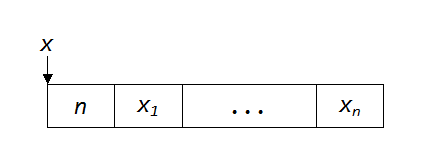
\includegraphics[width=0.5\textwidth]{tuple.png}\\
  \caption{memory map for tuple $x=(x_1,\ ...,\ x_n)$}\label{fig:digit}
\end{figure}

\begin{figure}
  \centering
  % Requires \usepackage{graphicx}
  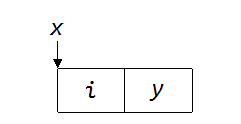
\includegraphics[width=0.28\textwidth]{tag.png}\\
  \caption{memory map for tagged value $x=\textsf{in}_i\ y$}\label{fig:digit}
\end{figure}

As is shown in Figure 8, a tuple with $n$ components will occupy $n+1$ memory
cells. The first cell is to store the length of the tuple, the rest $n$ cells
store the component values in order. In this lab, each cell is constraint to be 4 Bytes.
In this way, \texttt{allocTuple(n)} will allocate a memory space of $4*(n+1)$ Bytes
and store the value $n$ in the first cell. Finally it returns a pointer to
the first cell. The value of the components will be loaded later via this
pointer.

Note that we will never visit a tuple with the length of 0, so we can simply
output "\texttt{x=0}" instead of "\texttt{x=allocTuple(0)}".

As shown in Figure 9, a tagged value $\textsf{in}_i\ y$ takes two memory
cells. The first cell is to store the tag value $i$ (1 or 2), while the second
one for the value to be tagged.
In this way, \texttt{allocTag(i)} will allocate a memory space of 8kb
and store the tag value $i$ in the first cell. And finally it will return a pointer to
the first cell. The value $y$ will be loaded later via this pointer.\\

\noindent{
\fbox{%
\parbox{\textwidth}{%
 \textbf{Exercise 4}. Finish function \texttt{allocTuple} and \texttt{allocTag}
  in file \texttt{test/runtime.c}. You should allocate memory space and do some
  initializations according to Figure 8 and 9.
  Finally you should return a pointer to the proper memory address.

  $\ \ $We have provided some examples in folder \texttt{example} to test your
  implementation for the runtime system.
}
}
}

$\ $\\

\noindent{
\fbox{%
\parbox{\textwidth}{%
 \textbf{Exercise 5}.  Finish the \texttt{dump2file'} functions for
 expressions and bindings, in file \texttt{machine.sml}.
 The \texttt{dump2file} functions will output a syntax term as C code.

 $\ \ $ This completes the code generation procedure. After you have compiled
 everything (in SML/NJ), you can test your code by taping "\texttt{Main.main(t, "fname")}".
 Where \texttt{t} is MLAst.t, and \texttt{fname} is the prefix of the output files.
 If everything is correct, an executive file will be generated (you need to install
 a C compiler such as gcc, see \texttt{Main.sml}).

 $\ \ $ The examples in folder \texttt{example} may offer you some clues.

 $\ \ $ We have provided some test cases in \texttt{test.sml}. Yet you may want to write
 some of your own examples to test your Monkey compiler.
}
}
}\\

\end{document}
